% SC4051 --- Chapter 1: Foundations of Distributed Systems (0->100)
\chapter{Foundations: Fallacies, Models and the CAP Landscape}
\label{ch:foundations}

\begin{quote}
\emph{``A distributed system is one in which the failure of a computer you didn't even know existed can render your own computer unusable.''} --- Leslie Lamport. This chapter names the forces that make that quote true and gives you the vocabulary to reason about them.
\end{quote}

\noindent\fbox{\parbox{\dimexpr\linewidth-2\fboxsep-2\fboxrule}{%
\textbf{From zero: no distributed-systems background assumed.} We start from a single program on one machine and ask what changes when we add a network, a second machine, and the possibility that either or the network can fail. Every term is defined on first use. We move from intuition to formal models to the CAP theorem.}}
\vspace{0.4em}

\section*{Learning Outcomes}
After this chapter you will be able to:
\begin{enumerate}[label=(L\arabic*)]
    \item list and explain the eight fallacies of distributed computing with concrete failure examples;
    \item distinguish the synchronous, partially synchronous and asynchronous timing models;
    \item define crash-stop, crash-recovery, omission and Byzantine failure models;
    \item state and prove the CAP theorem and explain its practical scope;
    \item classify a system (DNS, ZooKeeper, Dynamo) by its consistency--availability trade-off.
\end{enumerate}

% ============================================================
\section{Why Distribution Is Different}
\label{sec:why-distributed}
A single machine is deceptively simple: memory is shared, failure is total (it crashes or it does not), and there is one clock. Add a network and all three assumptions break. The network can drop, delay, duplicate or reorder messages. Machines fail independently. Clocks drift apart. What looks like a procedure call becomes a protocol with timeouts, retries and partial failure.

Peter Deutsch's \emph{eight fallacies of distributed computing} catalog the dangerous assumptions:
\begin{enumerate}[leftmargin=1.4em,itemsep=0.25em]
    \item The network is reliable.
    \item Latency is zero.
    \item Bandwidth is infinite.
    \item The network is secure.
    \item Topology does not change.
    \item There is one administrator.
    \item Transport cost is zero.
    \item The network is homogeneous.
\end{enumerate}
Each fallacy has bitten a real system. Fallacy~1: a mobile app that assumes TCP always delivers and loses orders on a tunnel handover. Fallacy~2: a chatty RPC loop that makes 100 sequential calls and turns 1\,ms per call into 100\,ms of user-visible latency. Fallacy~4: a flat internal network that assumed no attacker inside---until a compromised printer became a pivot.

The remedy is not to patch each fallacy but to design with them as premises: expect loss, account for latency, budget bandwidth, authenticate everything, handle reconfiguration, and embrace heterogeneity.

\begin{figure}[h]
\centering
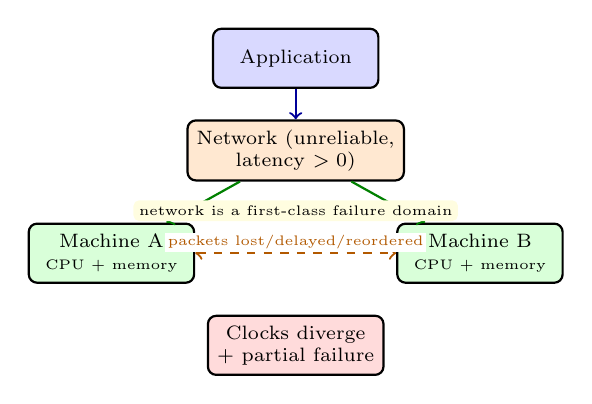
\begin{tikzpicture}[scale=0.90, every node/.style={font=\scriptsize},
  box/.style={draw,rounded corners=3pt,minimum width=2.1cm,minimum height=0.75cm,align=center,thick}]
\node[box,fill=blue!15] (app) at (0,2.2) {Application};
\node[box,fill=orange!18] (net) at (0,0.9) {Network (unreliable,\\latency $>0$)};
\node[box,fill=green!15] (m1) at (-2.6,-0.55) {Machine A\\{\tiny CPU + memory}};
\node[box,fill=green!15] (m2) at (2.6,-0.55) {Machine B\\{\tiny CPU + memory}};
\node[box,fill=red!14] (clk) at (0,-1.85) {Clocks diverge \\ + partial failure};
\draw[->,thick,blue!60!black] (app) -- (net);
\draw[<->,thick,orange!70!black,dashed] (m1) -- (m2) node[midway,above,font=\tiny,fill=white,inner sep=1pt] {packets lost/delayed/reordered};
\draw[->,thick,green!50!black] (net) -- (m1);
\draw[->,thick,green!50!black] (net) -- (m2);
\node[font=\tiny,align=center,fill=yellow!12,rounded corners=2pt,inner sep=2pt] at (0,0.05) {network is a first-class failure domain};
\end{tikzpicture}
\caption{From one machine to two: the network and independent clocks/failures become part of the model.}
\label{fig:dist-intro}
\end{figure}

% ============================================================
\section{System and Failure Models}
\label{sec:models}
A \emph{system model} fixes what we assume about processes, links and time; a \emph{failure model} fixes how things can break. Both bound what algorithms can guarantee.

\paragraph{Timing models.} \emph{Synchronous}: there are known bounds on processing time and message delay and clocks have bounded drift---rare in the Internet but useful for analysis. \emph{Asynchronous}: no bounds at all. Because FLP (Ch.~4) shows consensus is impossible in async with one crash, real systems assume \emph{partial synchrony}: bounds exist but are unknown or hold only eventually (Dwork--Lynch--Stockmeyer). Practical timeouts live here.

\paragraph{Failure models (ordered by severity).}
\begin{description}[leftmargin=1.2em,style=nextline]
    \item[Crash-stop (fail-stop)] A process halts and never recovers; others can detect it (eventually). Cleanest to reason about.
    \item[Crash-recovery] A process may crash and later restart with stable storage intact (write-ahead log survives). Most databases assume this.
    \item[Omission] Messages may be lost (send-omission or receive-omission) but processes do not lie.
    \item[Byzantine (arbitrary)] A faulty process may do anything---send conflicting messages, collude, act maliciously. Needed for open or adversarial settings.
\end{description}

\begin{definition}[Fail-stop vs.\ fail-recovery vs.\ Byzantine]
A \emph{fail-stop} process either follows its program or halts visibly. A \emph{fail-recovery} process may halt and later resume from stable storage. A \emph{Byzantine} process may deviate arbitrarily from its specification. Tolerating Byzantine faults with $f$ faults needs $n \ge 3f+1$ replicas (vs.\ $2f+1$ for crash faults).
\end{definition}

\begin{figure}[h]
\centering
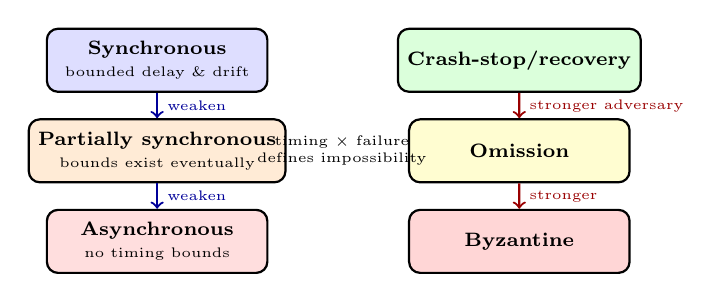
\begin{tikzpicture}[scale=0.92, every node/.style={font=\scriptsize},
  mod/.style={draw,rounded corners=4pt,minimum width=2.8cm,minimum height=0.80cm,align=center,thick}]
\node[mod,fill=blue!13] (sync) at (0,1.7) {\textbf{Synchronous}\\{\tiny bounded delay \& drift}};
\node[mod,fill=orange!16] (psync) at (0,0.45) {\textbf{Partially synchronous}\\{\tiny bounds exist eventually}};
\node[mod,fill=red!13] (async) at (0,-0.80) {\textbf{Asynchronous}\\{\tiny no timing bounds}};
\node[mod,fill=green!14] (crash) at (5.0,1.7) {\textbf{Crash-stop/recovery}};
\node[mod,fill=yellow!18] (omit) at (5.0,0.45) {\textbf{Omission}};
\node[mod,fill=red!16] (byz) at (5.0,-0.80) {\textbf{Byzantine}};
\draw[->,thick,blue!60!black] (sync) -- (psync) node[midway,right,font=\tiny] {weaken};
\draw[->,thick,blue!60!black] (psync) -- (async) node[midway,right,font=\tiny] {weaken};
\draw[->,thick,red!60!black] (crash) -- (omit) node[midway,right,font=\tiny] {stronger adversary};
\draw[->,thick,red!60!black] (omit) -- (byz) node[midway,right,font=\tiny] {stronger};
\node[font=\tiny,align=center] at (2.55,0.45) {timing $\times$ failure\\defines impossibility};
\end{tikzpicture}
\caption{Two orthogonal model dimensions: timing assumptions (vertical left) and failure severity (vertical right).}
\label{fig:models}
\end{figure}

Timing and failure together determine what is implementable. Example: perfect failure detection is possible in synchronous crash-stop but impossible in asynchronous---any timeout may confuse slowness with failure.

% ============================================================
\section{The CAP Theorem}
\label{sec:cap}
The CAP theorem (Brewer, 2000; Gilbert--Lynch, 2002) says a read/write register replicated over a network that can partition cannot be both \emph{linearizable} (consistent) and \emph{available} on every request during the partition. Formally, of Consistency, Availability and Partition-tolerance, you can have at most two---and since partitions happen, the real choice is CP vs.\ AP.

\begin{definition}[CAP properties for a read/write register]
\emph{Consistency} means linearizability: every read returns the most recent write in a global real-time order. \emph{Availability} means every non-faulty node returns a non-error response to every request. \emph{Partition tolerance} means the system continues despite arbitrary message loss between groups of nodes.
\end{definition}

\paragraph{Proof sketch (partition argument).} Partition nodes into $G_1$ and $G_2$ with all cross messages lost. Client $c_1$ writes $v$ to $G_1$; client $c_2$ concurrently reads from $G_2$. If the system is available, $G_2$ must answer. If it is consistent, it must return $v$, but it has no way to learn $v$ across the partition. So one property must be sacrificed. The system must either block/error (sacrifice availability) or return stale data (sacrifice consistency). \hfill$\square$

\begin{figure}[h]
\centering
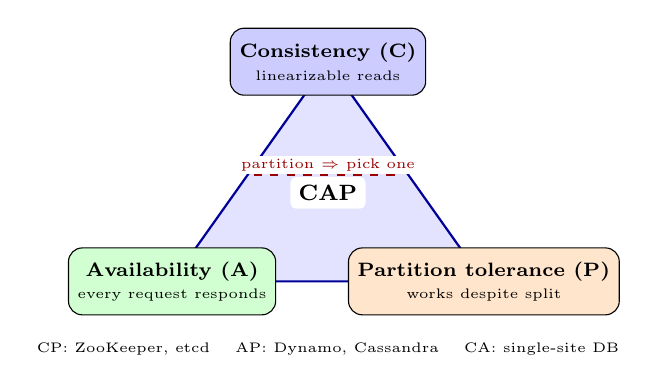
\begin{tikzpicture}[scale=0.90, every node/.style={font=\scriptsize}]
\coordinate (C) at (0,2.0); \coordinate (A) at (-2.2,-1.1); \coordinate (P) at (2.2,-1.1);
\fill[blue!11,draw=blue!60!black,thick,rounded corners=4pt] (C) -- (A) -- (P) -- cycle;
\node[draw,fill=blue!20,rounded corners=5pt,minimum width=2.45cm,minimum height=0.85cm,align=center] at (C) {\textbf{Consistency (C)}\\\tiny linearizable reads};
\node[draw,fill=green!18,rounded corners=5pt,minimum width=2.45cm,minimum height=0.85cm,align=center] at (A) {\textbf{Availability (A)}\\\tiny every request responds};
\node[draw,fill=orange!20,rounded corners=5pt,minimum width=2.45cm,minimum height=0.85cm,align=center] at (P) {\textbf{Partition tolerance (P)}\\\tiny works despite split};
\node[font=\footnotesize\bfseries,fill=white,rounded corners=2pt,inner sep=3pt] at (0,0.15) {CAP};
\draw[thick,red!60!black,dashed] (-1.05,0.40) -- (1.05,0.40) node[midway,above,font=\tiny,fill=white,inner sep=1pt] {partition $\Rightarrow$ pick one};
\node[font=\tiny,align=center] at (0,-2.05) {CP: ZooKeeper, etcd \quad AP: Dynamo, Cassandra \quad CA: single-site DB};
\end{tikzpicture}
\caption{CAP triangle: under a partition you must choose C or A. Real systems also tune latency vs.\ consistency within that choice.}
\label{fig:cap}
\end{figure}

\paragraph{CAP is not the whole story.} CAP talks about a single register under partition. Real trade-offs are finer: latency vs.\ consistency (PACELC), and many systems offer tunable consistency (read quorum $R$ + write quorum $W$ vs.\ $N$). Saying ``we are AP'' without stating which operations are available and with what staleness bound says little. Nevertheless CAP is the right first lens: it forces you to decide what happens when the network splits.

\begin{example}[Classifying systems]
DNS is AP: it stays available under partition but may serve stale records (TTL-based). ZooKeeper is CP: it refuses writes on the minority side to keep linearizability. Dynamo-style stores let you choose $R+W>N$ for strong consistency or $R+W\le N$ for availability and lower latency.
\end{example}

\begin{remark}[Availability vs.\ fault tolerance]
CAP's ``availability'' means every request to a non-failed node succeeds, which is stronger than ``the service as a whole stays up somewhere.'' Most ``highly available'' systems are CP per CAP but highly available in the colloquial sense via failover and retries.
\end{remark}

% ============================================================
\section{Abstractions: State Machine Replication}
\label{sec:smr}
The central abstraction for fault tolerance is \emph{state machine replication} (SMR): make $n$ replicas behave like one correct state machine by feeding them the same commands in the same order. If replicas start in the same state and apply deterministic commands in identical order, they stay identical---so the service survives $f$ faulty replicas.

SMR needs two ingredients: (1) a \emph{total-order broadcast} (all correct replicas deliver messages in the same order) and (2) deterministic execution. Consensus (Ch.~4) implements total order; replication protocols (Ch.~5) implement it efficiently.

A tiny simulation makes the idea concrete.

\begin{lstlisting}[language=Python]
# SMR intuition: deterministic replicas + total order => identical state
class Replica:
    def __init__(self, rid):
        self.id = rid
        self.state = {}          # key-value state machine
        self.log = []            # ordered command log
    def apply(self, cmd):
        # deterministic: same cmd on same state => same new state
        op, k, v = cmd
        if op == "put":
            self.state[k] = v
        elif op == "delete":
            self.state.pop(k, None)
        self.log.append(cmd)

# total-order broadcast delivers same sequence to every replica
commands = [("put","x",10), ("put","y",20), ("put","x",15)]
replicas = [Replica(i) for i in range(3)]
for cmd in commands:            # same order to all replicas
    for r in replicas:
        r.apply(cmd)

assert all(r.state == replicas[0].state for r in replicas)
print("all replicas converge:", replicas[0].state)
# {'x': 15, 'y': 20}  -- order matters: x=15 not 10
\end{lstlisting}

Change the delivery order on one replica and the states diverge---that is the failure SMR prevents. The rest of this book is largely about how to achieve total order under failures, asynchrony and scale.

\begin{example}[Replicated counter with lost update]
Two clients concurrently increment a counter at replicas $R_1,R_2$ without total order: $R_1$ sees $inc$ then $inc$ (value $2$), $R_2$ sees the two $inc$ in opposite order but still $2$---commutative here. Replace $inc$ with $x:=x+1$ plus a conditional $if~x>5~then~alert$: order now matters for whether the alert fires. SMR ensures every replica evaluates the condition in the same order, so alerts are consistent.
\end{example}

\begin{remark}[Why SMR needs consensus]
Total-order broadcast is equivalent to consensus: deciding the $k$-th log entry is a consensus instance. Hence FLP (Ch.~4) applies---SMR is impossible in pure async with one crash, which is why practical SMR (Raft, Paxos, Viewstamped Replication) assumes partial synchrony and elects a leader.
\end{remark}

% ============================================================
\section{Exercises}
\label{sec:ch01-exercises}
\begin{enumerate}[label=E1.\arabic*, leftmargin=*, itemsep=0.6em]
    \item \textbf{Fallacies in the wild.} For each of fallacies 1, 2 and 4, describe a concrete user-visible failure in a mobile payment app and a design mitigation (timeout, retry budget, mTLS, etc.). Why does retrying blindly on an idempotent-unsafe operation make fallacy~1 worse?
    \item \textbf{Timing models and FLP.} Explain why a 100\,ms client timeout cannot implement perfect failure detection in an asynchronous network. How does partial synchrony rescue the argument? State the FLP impossibility in one sentence.
    \item \textbf{CAP proof reconstruction.} Reconstruct the Gil\-bert--Lynch partition argument for a single register. Extend it to argue that no algorithm can guarantee both linearizability and availability for \emph{every} operation during a partition, even with unbounded retries.
    \item \textbf{Failure model hierarchy.} Order crash-stop, crash-recovery, omission and Byzantine from weakest to strongest adversary. For each step, give an example fault the stronger model captures but the weaker does not. Why does Byzantine tolerance need $n\ge 3f+1$?
    \item \textbf{Classify and tune.} Classify DNS, etcd/ZooKeeper and Dynamo/Cassandra on the CAP triangle. For a Dynamo-style store with $N=3$, enumerate $(R,W)$ pairs giving strong consistency vs.\ eventual consistency and compute the read/write availabilities under one replica down.
\end{enumerate}

% ============================================================
\section*{Chapter Notes}
Lamport's definition and Deutsch's fallacies are collected in Rotem-Gal-Oz, \emph{Fallacies of Distributed Computing} (2006). System models follow Cachin--Guerraoui--Rodrigues, \emph{Introduction to Reliable and Secure Distributed Programming} (2011, Ch.~2) and Coulouris et al., \emph{Distributed Systems} (5th ed.). CAP: Brewer's PODC keynote (2000) and Gilbert--Lynch, ``Brewer's conjecture and the feasibility of consistent, available, partition-tolerant web services'' (SIGACT News, 2002). PACELC: Abadi (2012). SMR: Schneider, ``Implementing fault-tolerant services using the state machine approach'' (ACM Comp.~Surv., 1990).

% End of Chapter 1
